\documentclass[10pt, twoside]{article}   	% use "amsart" instead of "article" for AMSLaTeX format
\usepackage[innermargin=3in, top=0.75in]{geometry}                		% See geometry.pdf to learn the layout options. There are lots.
\usepackage[english]{babel}
\geometry{a4paper}                   		% ... or a4paper or a5paper or ... 
%\geometry{landscape}                		% Activate for for rotated page geometry
%\usepackage[parfill]{parskip}    		% Activate to begin paragraphs with an empty line rather than an indent
\usepackage{graphicx}				% Use pdf, png, jpg, or epsß with pdflatex; use eps in DVI mode
\usepackage{fontspec}
\setmainfont{Arial}
					
\linespread{1.1}			% TeX will automatically convert eps --> pdf in pdflatex		
\usepackage{amssymb}
\usepackage{eurosym}
\usepackage{colortbl}
\usepackage{titlesec}
\titleformat{\section}[block]%
  {\normalfont\scshape\filright}%
  {\makebox[2em][l]{\thesection}}%
  {1em}
  {}[\color{blue}{\titlerule}]
\titlespacing{\section}{-3em}{3.5ex plus 1ex minus .2ex}{2.3ex plus .2ex}
\titleformat{\subsection}[block]%
  {\color{blue}{\normalfont\scshape\filright}}%
  {\makebox[2em][l]{\color{blue}{\thesubsection}}}%
  {1em}
 {}
 


\title{DragPanels}
\author{Stephan J.C. Eggermont, Sensus}
\begin{document}
\setlength{\parindent}{0pt}
\maketitle
\begin{quote}
\em
DragPanels demonstrates how to make widgets that support click, double-click, drag-and-drop
and context menus in Morphic. This is shown with a color panel and an avatar panel.
Morphic is a powerful graphics environment, used in Self, Squeak, Cuis and Pharo.
\end{quote} 
%%%%%%%%%%%%%%%%%%%%%%%%%%%%%%%%%%%%%%%%%%%
\section{A color and avatar panel}
\begin{figure}[htb]
\begin{center}
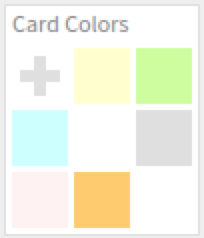
\includegraphics[width=100pt]{CardColors.png}
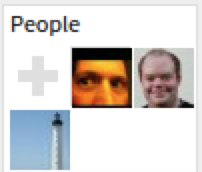
\includegraphics[width=100pt]{Avatars.png}
\caption{The panels}
\label{1stIteration}
\end{center}
\end{figure}
The first iteration (Figure \ref{1stIteration})  shows two panel windows that
stay in front of other windows. They can be moved around  by dragging
the title bar part. The plus symbol can be clicked to add new elements
to the panel. Each element is a square of 30*30 pixels. An element can 
start a drag action where a copy of the element is dragged to a Morph that
wants to receive it. The default action for dragging a color is setting the color
of the Morph, for dragging an avatar it is setting the email.


%%%%%%%%%%%%%%%%%%%%%%%%%%%%%%%%%%%%%%%%%%%
\section{Loading the code}
The code can be found on www.smalltalkhub.com, in the repository StephanEggermont/DragPanels
Open the Monticello Browser. Add a new repository of type smalltalkhub.com. 
The owner is StephanEggermont, the project is DragPanels. User and password are only needed
when you want to commit changes to the repository. Open the repository and load the latest version of
DragPanels.


\end{document}  